\documentclass[conference]{IEEEtran}
%\usepackage[titletoc]{appendix}
\usepackage{gensymb}
\usepackage{float}
\usepackage{graphicx}
\usepackage[pdftex,
			final,
            pdfauthor={Adrien Raulot and Luc Gommans},
            pdftitle={DNS bitsquatting in 2018},
            pdfkeywords={dns bit flip error domain squatting}]{hyperref}
\usepackage{wrapfig}
\usepackage{booktabs}
\hypersetup{
	colorlinks=true,       % false: boxed links; true: coloured links
	linkcolor=blue,        % colour of internal links
	citecolor=blue,        % colour of links to bibliography
	filecolor=magenta,     % colour of file links
	urlcolor=blue
}

\usepackage[
    backend=bibtex,
    style=numeric,
    sorting=none,
    maxcitenames=2
]{biblatex}

\usepackage{listings}
\lstset{breaklines, basicstyle=\small\ttfamily\footnotesize\bfseries}

\bibliography{references.bib}

\begin{document}

\title{DNS bitsquatting in 2018\\\vspace{5mm} \large  \today}
\author{
\IEEEauthorblockN{Adrien Raulot}
\IEEEauthorblockA{
Security and Network Engineering \\
University of Amsterdam \\
adrien.raulot@os3.nl}
\and
\IEEEauthorblockN{Luc Gommans}
\IEEEauthorblockA{
Security and Network Engineering \\
University of Amsterdam \\
os3-ot@lucgommans.nl}
}
\maketitle
\thispagestyle{plain}
\pagestyle{plain}

\begin{abstract}

	In this paper we will investigate the current state of random DNS bit
	flips. While random bit errors in a single machine are not very common, the
	number of DNS queries performed worldwide is extremely large. Such an error
	might lead one to query for a domain name, and subsequently connect to the
	resulting IP address, which one never intended to connect to. We find that
	these errors are hard to reproduce and do not seem to be very common when
	observing traffic to bitsquat domains registered for this experiment.

\end{abstract}

\section{Introduction}

The vast majority of internet-connected computers perform DNS requests during
conventional use. Because the requests are so ubiquitous, there is reason to
suspect that sometimes, due to random variations, errors might naturally occur.
When an error occurs, one might query for and subsequently connect to a domain
which one never intended to communicate with.

In this paper we will investigate likely causes for bit flips in desktop
computers and attempt to determine whether the resulting attack, bitsquatting,
is still viable.

In the next section, we will define our research questions, followed by ethical
considerations in Section \ref{sec:ethics}. In Section \ref{sec:relwork} we
discuss previous work in this area. In the following three sections we will
describe our experiments and give the results: Section \ref{sec:exp1} describes
our experiment trying to cause bit flips by applying heat, \ref{sec:exp2}
describes bitsquatting domains we registered and monitored, and \ref{sec:exp3}
describes trying to cause bit flips using rowhammer. The results are briefly
discussed in Section \ref{sec:disc}. Finally, a conclusion is drawn in Section
\ref{sec:conc} and possible future work is discussed in section
\ref{sec:futwork}.


\section{Research Questions}\label{sec:researchq}

Our main research question is:
{\it Is bitsquatting a viable attack?}

\vspace{0.1cm}

\noindent{} This main research question divides in four sub-questions:

\begin{enumerate}
    \item What could a bitsquatting attack be used for?
	\item What circumstances cause random bit errors?
	\item Can we detect random bit errors currently occurring around the world?
	\item Are organisations mitigating the risk by preemptively purchasing
	      bitsquat domains?
\end{enumerate}

One important exclusion is network equipment. In this work, we only looked at
bit flips occurring on a common computer. Mobile equipment is only partially
targeted: to answer the third sub-question, we purposefully registered a domain
that is popular on mobile devices, but we did not ourselves attempt to trigger
memory corruption on a mobile device. If this occurs a lot on mobile devices,
we should observe a larger number of hits on that domain.


\section{Ethical Considerations}\label{sec:ethics}

Most of our work will focus on attempting to find causes of random bit errors.
However, in order to learn whether random bit errors are currently occurring in
practice, we will need to work with real domains and user data. This data is
kept confidential and will be destroyed after completion of the project. The
domains we register will not be used for anything other than determining
whether this is the result of a random bit error.


\section{Related Work}\label{sec:relwork}

In 2011, Artem Dinaburg presented for the first time the bitsquatting attack at
the DEFCON 19 security conference. In his
white paper\cite{dinaburg2011bitsquatting}, he describes bitsquatting as an
attack relying on random bit errors to redirect connections intended for
popular domains to domains registered by malicious entities. Since 2011, very
few research papers have been published about bitsquatting, hence this
research. Another research from 2011 by Nick et
al.\cite{nikiforakis2013bitsquatting} showed that bitsquatting was still
popular by monitoring newly registered bitsquat domains over a period of
270 days. In this period, a total of 5 366 different bitsquat domains were
registered, targeting 491 out of the Alexa top 500 domains.

\section{Experiment 1: Heating}\label{sec:exp1}

Although random bit flips are theoretically possible, the unlikeliness of a bit
flip in practice is important. Bit flips are soft errors, which are more likely
to occur in certain circumstances such as high temperature, low voltage, high
speed, alpha particles, cosmic rays, and others. This not only may have an
impact on the applications running on a system, but also raises security
concerns as attacks, such as the bitsquatting attack we describe in this paper
may take advantage of soft errors. During this research, we mainly focused on
producing soft errors in memory modules, although we also tested and monitored
the hard disk and the network for bit flips. Nowadays, Error-Correcting Code
(ECC) memory is commonly used in most computers where data corruption has a
large impact.

From the different fault injection techniques known to
exist\cite{barenghi2012fault}, we decided to use heat. This technique is
realistic of situations where desktop computers, servers and smartphones are
impacted by high temperatures and it is a relatively cheap technique to set up.
Because this technique could damage the hardware, we were careful to place the
disposable hardware in a safe environment and constantly monitor the
temperature. The latter, however, has been more difficult than we expected, as
we were not able to retrieve thermal values from the system. To remedy this, we
monitored the hard drive temperature as an indicator and manually measured the
temperature of the CPU and memory with a infrared temperature sensor gun.

We acquired a disposable desktop to experiment on and implemented three types
of test program\footnote{\url{https://github.com/lgommans/dns-bitsquatting/}}
to monitor bit flips:

\subsection{Memory test}

Our memory tester (Appendix \ref{Apdx-memory}) retrieves $(2^{12})-1$ bytes of
random data from \texttt{/dev/urandom} to use as random pattern. We configure
it to allocate 95\% of free memory, which it fills with this random pattern.
The amount of random bytes is chosen to explicitly not align to a memory page,
so that each page contains a new byte as first byte. A few redundant copies of
the correct pattern are kept separately.

After writing the pattern to the allocated memory, which consists of several
gigabytes so it cannot still be in CPU caches, we read the data again
sequentially and compare it against our pattern. We also make sure that the
pattern's copies are all equal.

After a few iterations, the random pattern is refreshed by reading new data
from \texttt{/dev/urandom}. If some patterns are more susceptible to
alterations than others, this should hopefully reveal that. Upon discovery of
an error, both the correct pattern and the pattern which we found instead are
logged.

\subsection{Disk test}

The disk test (Appendix \ref{Apdx-disk}) is similar to the memory test because
it also reads an uneven number of bytes from \texttt{/dev/urandom} and writes
that to a large file on disk. Here, too, we made sure that the file is large
enough not to fit in memory caches, and the pattern is refreshed after a few
iterations of writing and reading.

The main difference is that we do not keep redundant copies of the correct
pattern, as we are not attempting to detect memory corruption here. Any memory
corruption should be evident from the other program.

\subsection{Network test}

The network test (Appendix \ref{Apdx-network}) consists of two parts: a
transmitter and a receiver. We used a server (in the same building) to transmit
the data, and ran a receiver on the experimental hardware. The packets
transmitted are based on UDP, containing 1200 bytes payload. The first byte is
a tracking number: it will increment every time the payload changes. The last
32 bytes are a SHA-256 hash of the rest of the payload. Finally, the remainder
of the payload is, again, data read from \texttt{/dev/urandom}, and is changed
every 30 seconds.

The incremental number allows us to do a byte-by-byte check of the data, to
compare it against the previously received packets. If it is unequal, we know
that the payload changed and that we should recompute the hash. If the data was
not equal, the hash would also be recomputed because this should no longer
match. If it does not match, we log the last known correct contents and the
corrupted contents.

Data was transmitted at a rate of about 800 megabits per second (bursting 50
packets and then calling \texttt{nanosleep}). We checked for packet loss, and this was
low. This only occurred when the target system was too busy to drain its
receive buffer, and was not caused by network equipment. We consider this to
have no impact on our results.

\subsection{Desktop setup}\label{desktop-setup}

The desktop contains $2\times2$GB DDR2 RAM memory, an Intel Pentium D processor
and a 2TB Hitachi hard disk drive. More recent hardware was not considered
disposable by the university and therefore off limits for any sort of
experiment. The only alternative was an old server with ECC memory, which we
considered unfit for our purpose. Our CPU did not seem to contain a readable
temperature sensor: online we find many posts of users, on both Linux-based and
Windows operating systems, who find that they are unable to read the
temperature sensor. To have some notion of the machine's temperature, we used a
handheld infrared thermometer and the hard drive temperature.

In the machine, we created an isolated air inlet for the power supply unit
(PSU) and otherwise taped off all air intakes and outtakes. Aside from the PSU,
the CPU fan is the only fan in the system, which we left plugged in: this
circulates the hot air through the case and heats up other components such as
the memory.

During the tests, we run the three scripts in parallel. The CPU is a dual core
without Hyper-threading, so our network receive and RAM test scripts could run
in parallel at nearly full speed. The disk test script also ran at full speed,
since the majority of the time was spent on I/O. Running all scripts in
parallel also had the effect of putting the system under full load, generating
a lot of heat.

\subsection{Experiment 1: Results}\label{sub:exp1r}

During the experiment, we examined the logs periodically to see that the
experiments were running correctly and to see whether any bit flips had
manifested. The machine became less responsive at very high temperatures, but
at no point did any bit flips occur. Because we also could not read the current
CPU frequency, we do not know whether it throttled back. When measuring the
temperature of the components after this test, we measured 93\degree{}C on the
CPU cooler, 59\degree{}C on the hard drive (internal sensor) and 65\degree{}C
on the RAM memory.

Because the machine did not reach thermal cut-off temperature and did not
produce any bit flips yet, we then covered it with a cloth to prevent heat from
dissipating through the metal cover. While this had a bigger impact on the
overall internal temperature, raising the hard drive and RAM memory by almost
10\degree{}C, we were not able to produce any bit flips or reach cut-off
temperature.

Finally, in a third setup, we attempted heating the memory modules with a hair
dryer, similar to the memory corruption experiments described by Govindavajhala
and Appel\cite{jvm}. This had to be done with the case open, thus only heating
the memory and nearby components, but as Govindavajhala and Appel described
that similar memory to ours would start producing errors at 80--100\degree{}C,
we thought it worthwhile to focus on the RAM only. See figure
\ref{fig:hairdryer} for the experimental setup. This experiment was halted when
the hair dryer started melting, the thermometer started giving incorrect
readouts because it had heated up itself, and the computer continued to run
without any issues.

\begin{figure}
	\centering
	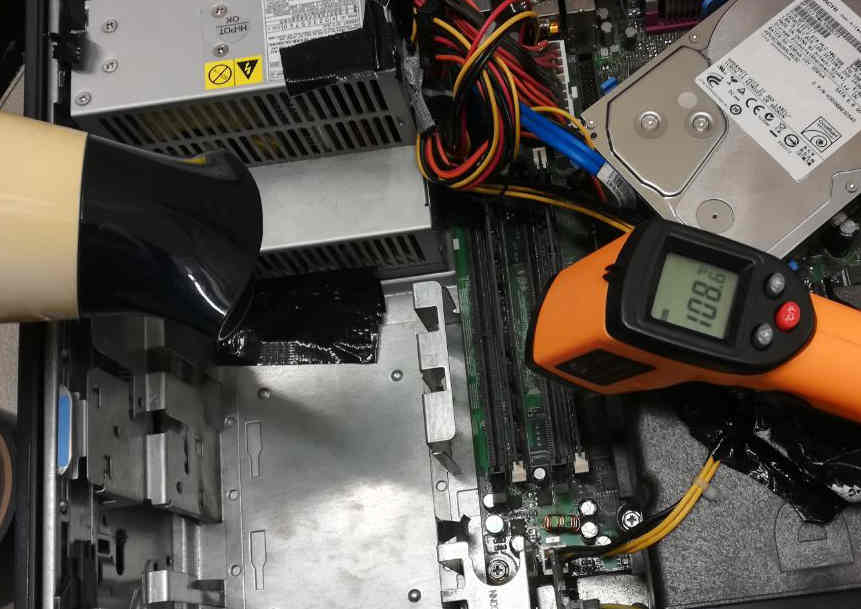
\includegraphics[width=0.49\textwidth]{hairdryer.jpg}
	\caption{Third experimental setup}
	\label{fig:hairdryer}
\end{figure}


\section{Experiment 2: Bitsquatting}\label{sec:exp2}

For our second experiment, we registered and monitored 5 domains:

\begin{itemize}
  \item \texttt{eoogle.be.}
  \item \texttt{eoogle.nl.}
  \item \texttt{eoogle.co.uk.}
  \item \texttt{whatsapx.net.}
  \item \texttt{a9u9h.nl.}
\end{itemize}

The latter is a control domain, registered to be able to see the difference
between a bitsquat domain and any other, unlisted domain. We picked the
name using a random number generator to make sure users did not stumble upon it
by accident. The name is short, so that it can be brute-forced by NSEC3 walks
(the \texttt{.nl} zone is DNSSEC-enabled). If our other domains are being found
via this method, then we will also see this on our control domain, and we know
that this traffic does not originate from random bit flips.

The bitsquat domains were chosen because we expect they get a lot of hits, and
because they should give a diversity of devices. For example, the WhatsApp
mobile application uses \texttt{whatsapp.net} rather than
\texttt{whatsapp.com}.

Table \ref{tab:bits} shows which bits were flipped for each domain.

\begin{table}[H]
  \centering
  \caption{Bitsquat vs. original domain names}
  \label{tab:bits}
  \begin{tabular}{|l|l|l|}
    \hline
    \textbf{Domain}   & \textbf{Bits} \\ \hline
    eoogle   & 01100101... \\ \hline
    google   & 011001\textbf{1}1... \\ \hline
    whatsapx & ...01111000 \\ \hline
    whatsapp & ...0111\textbf{0}000 \\ \hline
   \end{tabular}
\end{table}

We noticed that for many domains which we would have liked to register, such as
bitsquats of \texttt{google.com} or \texttt{facebook.com}, the domains were
already occupied. For \texttt{google.com}, many of the domains are owned by
Google, but a few are not. Generating bitsquat domains is not difficult and
domains are not expensive, so we assume this was not an attempt at preventing
bitsquatting. For \texttt{facebook.com}, the situation is reversed: some are
owned by Facebook, and many are owned by external parties. Many of the bitsquat
domains lead to websites with advertisements. For other popular domains, we
notice similar patterns. This answers one of our research questions: companies
do not seem to be trying to prevent bitsquatting.

To gather the results for the domains we registered, we ran a DNS server for
all domains. For each domain, we returned a unique IP address of ours.
Hypothetically, we would see a client with a random bit error query for
\texttt{e19.whatsapx.net}, give it the IP address \texttt{145.100.108.252}, and
then observe it attempting to build a TCP connection with that IP address on a
port used by WhatsApp.

We used tcpdump's pcap-writing functionality to monitor this usage. Each of the
used IP addresses referred to the same server, making monitoring easier.


\subsection{Experiment 2: Results}\label{sub:exp2r}

The control domain received 3 500 hits from the registrar (SIDN) and partners
(OpenIntel). These queried for various record types for the domain and the
subdomains \texttt{www}, \texttt{\_dmarc} and \texttt{\_domainkey}.

The other domains got many hits. It appears that \texttt{.co.uk} domains are
publicly listed, as we received 52 700 unsolicited queries of various types (A,
AAAA, TXT, NS, MX, etc.). In contrast, \texttt{eoogle.be} saw 12 000 queries
and \texttt{eoogle.nl} saw 6 600.

In 2011, Dinaburg\cite{dinaburg2011bitsquatting} recorded 52 000 bitsquat
requests over a period of 7 months, using 29 domains. This comes down to about
8.4 requests per domain per day. Perhaps memory got less error-prone to the
extent that the increased usage of the internet since 2011 is negated, but that
seems doubtful. We should probably see at least an equal number of requests.
However, to find those within a total of 169 700 queries, turned out to be
quite difficult.

The results were loaded into a relational database for easier querying. We
filtered the data in various ways, such as only listing queries from IP
addresses that were seen only once (since those errors are supposed to be rare)
and were querying for a normal record type, such as A or AAAA. Investigating
this list by looking in the gathered pcaps, we find that these IP addresses
never follow up on the response they were given. In some cases, a completely
different IP address (sometimes from a different continent, compared to the
original address) immediately attempts to contact the IP address that we
returned. They often attempt to contact a random port, not used by the service
we are bitsquatting.

Another query we attempted filters on addresses which we only saw 1--4 times
and which queried for both the A and AAAA records. It is typical to query for
both, so a legitimate client should do that. This yielded only 58 records: some
from Google and some from DigitalOcean, but also some promising-looking
resolvers such as from Level3. Looking in pcaps again, we found no normal
follow-up traffic.

No matter how we cut or slice the dataset, in no case does an IP address show
both normal resolver behaviour and follow up with normal traffic. Some of the
ones without follow-up traffic could be caused by bit errors, as a response for
the wrong query name might be ignored (if a resolver queries for A and gets an
answer for B, it might ignore it depending on where the error occurred), but
we cannot verify this with any certainty.

We also noticed a large number of queries from many different IP addresses at
Amazon AWS and Google (presumably their AWS-equivalent), as well as various
research institutes and other services which advertise themselves as DNS
scanners.

\section{Experiment 3: Rowhammer}\label{sec:exp3}

High memory densities create an increased rate of electromagnetic interactions
between memory cells\cite{kim2014flipping}. Our third experiment focuses on
accidental or intentional leaking of currency into nearby cells, possibly
causing bit flips that way.

We first needed to assert how likely this is when one tries to do this
intentionally. To test this, we used two different test suites: one by the team
at Google's Project
Zero\footnote{\url{https://github.com/google/rowhammer-test}} and one by Gruss
et
al.\cite{gruss2016rowhammer}\footnote{\url{https://github.com/IAIK/rowhammerjs}}.
From the latter, we ran the general tests, the specific one for our Ivy Bridge
hardware, and the JavaScript-based one.


\subsection{Experiment 3: Results}\label{sub:exp3r}

The experimental hardware for experiment 1 (Section \ref{desktop-setup}) is
definitely not vulnerable, as the memory is too old. On our server and
workstations, the test suites did not manage to trigger the attack. It appears
that our hardware is not vulnerable.


\section{Discussion}\label{sec:disc}

Since part of our bitsquat domains ingress traffic was coming from
research institutes such as universities or laboratories and there is no easy
way to prevent this, it was very difficult to filter the noisy traffic out from
the legitimate traffic caused by bit flips. This also poses a design problem
about bitsquatting experiments, the fact that researchers monitoring the
Internet for bitsquat domains used by attackers end up querying
bitsquat domains set up by other researchers. Moreover, traffic monitoring
experiments should be carried out during a longer period, as three weeks is not
enough to be able to clearly identify interesting traffic due to bit flips.


\section{Conclusion}\label{sec:conc}

We conclude that DNS errors due to bit flips are rare, as we have not been able
to find any while observing bitsquat domains for several weeks, nor have we
been able to produce any bit errors ourselves even under unrealistically
hostile circumstances. Our hardware proved to be very resilient to heat.

Organisations do not seem to be preemptively buying bitsquat domains to
mitigate the attack. It is likely that large corporations such as Google would
have looked into this after the publication by Dinaburg in 2011, and would have
registered the domains if it had been deemed a reasonable attack vector.

Finally, our hardware also proved to be resilient to rowhammer. Even if there is
software which could accidentally cause cell leakage and corrupt DNS (or other)
memory this way, the hardware itself still needs to be vulnerable.


\section{Future Work}\label{sec:futwork}

We expect the following areas to be interesting as future work:

\subsection{Different hardware}

Similar experiments could be run on mobile devices, which are smaller and have
higher memory densities. It is likely that there is much more electronic
interference which could cause bit flips.

The hardware we used was fairly old (2005). Modern hardware might give
different results.

Finally, the hardware we used was not allowed to be left turned on unattended.
The room available for our experiment was unsuitable for doing work other than
attending the computer as it ran, which severely limited how many hours we were
able to run the experiments for. Being able to leave the system running
unattended and over night, or perhaps running more machines in parallel, would
yield much more data to work with.


\subsection{Other causes of bit flips}

In our experiments, we focused mainly on heat. Our hardware proved not to be
vulnerable to rowhammer. Our experiments could be run with interference other
than heat, such as electromagnetic interference.

On hardware vulnerable to rowhammer, it would also be valuable to experiment
with software that might accidentally trigger cell bleeding.

\subsection{Other DNS-related attacks}

Stucke\cite{suffixpath} described an attack relating to DNS search paths, where
he would register domains mistakenly used by clients, for example by mistakenly
adding the search path to what was supposed to be an FQDN. For example, we have
observed strange behaviour in unrelated experiments, where servers would query
for \texttt{eno2} (an interface name) and \texttt{eno2.<search\_path>}. If
someone were to register a domain which is unintentionally queried for, they
would be able to capture requests from such a system.


\printbibliography

\begin{appendices}

\section*{Appendices}

N.B. The code is also available on our Github: \\
\url{https://github.com/lgommans/dns-bitsquatting/}

\section{Memory test}\label{Apdx-memory}
\begin{lstlisting}[language=C]
#include <stdio.h>
#include <stdlib.h>
#include <string.h>
#include <sys/types.h>
#include <sys/stat.h>
#include <fcntl.h>
#include <unistd.h>

#define RANDOM_SRC "/dev/urandom"
#define P_LENGTH 4 * 1000
#define SET_ITERATIONS 1
#define READ_ITERATIONS 1

void prnt(char *s, int l) {
  for (int i = 0; i < l; i++)
    printf("%x ", s[i]);
}

int main(int argc, char** argv) {
  long alloc_size = strtol(argv[1], NULL, 10);
  char *s = (char*)malloc(sizeof(char) * alloc_size);
  char p1[P_LENGTH], p2[P_LENGTH], p3[P_LENGTH], pa[P_LENGTH];
  int i = 0;
  long shift = 0;
  int rdm = open(RANDOM_SRC, O_RDONLY);
  if (rdm < 0) {
    return 1;
  }

  if (read(rdm, pa, P_LENGTH) < 0) {
    return 3;
  }

  while (1) {
    if (shift + P_LENGTH >= alloc_size) {
      shift = 0;
      if (i == SET_ITERATIONS + READ_ITERATIONS) {
        printf("New random values\n");
        i = -1;
        if (read(rdm, p1, P_LENGTH) < 0 ||
            read(rdm, pa, P_LENGTH) < 0) {
          return 2;
        }
        memcpy(p2, p1, P_LENGTH);
        memcpy(p3, p1, P_LENGTH);
      }
      else {
        if (i == SET_ITERATIONS) {
          printf("Set round complete. Reading...\n");
        }
      }
      i++;
    }

    if (i < SET_ITERATIONS) {
      memcpy(s + shift, pa, P_LENGTH);
      memcpy(s + shift, p1, P_LENGTH);
    }
    else {
      if (memcmp(s, p1, P_LENGTH)) {
        printf("Bit flip detected. Should have been:\n");
        prnt(p1, P_LENGTH);
        printf("\nBut was instead:\n");
        prnt(s, P_LENGTH);
        printf("\n");
        if (memcmp(p1, p2, P_LENGTH) || memcmp(p2, p3, P_LENGTH) || memcmp(p1, p3, P_LENGTH)) {
          printf("And the pattern was corrupted.\n");
          continue;
        }
      }
    }
    shift += P_LENGTH;
  }
  free(s);
  close(rdm);
}
\end{lstlisting}

\section{Disk test}\label{Apdx-disk}
\begin{lstlisting}[language=Python]
#!/usr/bin/env python3

path = '/dev/sdd'
filesize = 400e9
patternlength = 4096 - 1


import os, binascii

testrunnum = 0

while True:
  if testrunnum % 4 == 0:
    print('Generating new pattern.')
    pattern = os.urandom(patternlength)

  testrunnum += 1

  f = open(path, 'wb')
  wrotebytes = 0
  while wrotebytes < filesize - patternlength:
    f.write(pattern)
    wrotebytes += patternlength
  f.close()

  f = open(path, 'rb')
  readbytes = 0
  while readbytes < filesize - patternlength:
    r = f.read(patternlength)
    readbytes += patternlength
    if r != pattern:
      print('Changed! Original:')
      print(binascii.hexliy(pattern))
      print('Result:')
      print(binascii.hexliy(r))
      print('-------------')

  print('Test run {} complete.'.format(testrunnum))
\end{lstlisting}

\section{Network test}\label{Apdx-network}
\subsection{Transmitter}
\begin{lstlisting}[language=C++]
#include <sys/socket.h>
#include <netdb.h>
#include <memory.h>
#include <iostream>
#include <ctime>
#include <openssl/sha.h>
#include <sys/stat.h>
#include <fcntl.h>
#include <unistd.h>
#include <stdlib.h>

using namespace std;

void sha256(const unsigned char* str, int len, unsigned char* hash)
{
  SHA256_CTX sha256;
  SHA256_Init(&sha256);
  SHA256_Update(&sha256, str, len);
  SHA256_Final(hash, &sha256);
}

int resolvehelper(const char* hostname, int family, const char* service, sockaddr_storage* pAddr)
{
  int result;
  addrinfo* result_list = NULL;
  addrinfo hints = {};
  hints.ai_family = family;
  hints.ai_socktype = SOCK_DGRAM; // without this flag, getaddrinfo will return 3x the number of addresses (one for each socket type).
  result = getaddrinfo(hostname, service, &hints, &result_list);
  if (result == 0)
  {
    //ASSERT(result_list->ai_addrlen <= sizeof(sockaddr_in));
    memcpy(pAddr, result_list->ai_addr, result_list->ai_addrlen);
    freeaddrinfo(result_list);
  }

  return result;
}

int main(int argc, char** argv) {
  int evoevery = 60;  // Evolve (renew payload) every this many seconds
  int sendbytes = 1200;  // How many bytes UDP payload? (Hash is put in the last sendbytes-hashlen_bytes bytes.)
  int hashlen_bytes = 32;  // Length (in bytes) of the chosen hashing algorithm
  int errlimit = 5000;  // Die after this many errors
  int sleepDivider = 50;  // Only sleep every N transmissions, because the nanosleep call has an amazing amount of overhead, for something claiming to sleep some 'nanoseconds'...
  //int overhead = 18 + 20 + 8;  // Overhead for each transmitted packet, in bytes (eth,ip,udp)
  double bwcorrectionfactor = 0.93;

  if (argc != 4) {
    cout << "Usage: testnet <dst host> <port> <bandwidth-in-mbps>" << endl;
    return 1;
  }

  int mbitpersec = strtol(argv[3], NULL, 10);  // Bandwidth limit, in megabits. Note that tx rate is only evaluated once per evolution.
  int bwlimit = mbitpersec * 1e6 / 8;
  int errs = 0;
  int nextevo = 0;
  int result = 0;
  int sock = socket(AF_INET, SOCK_DGRAM, 0);

  sockaddr_in addrListen = {}; // zero-int, sin_port is 0, which picks a random port for bind.
  addrListen.sin_family = AF_INET;
  result = bind(sock, (sockaddr*)&addrListen, sizeof(addrListen));
  if (result == -1)
  {
    cout << "error n2";
    return 2;
  }

  sockaddr_storage addrDest = {};
  result = resolvehelper(argv[1], AF_INET, argv[2], &addrDest);
  if (result != 0)
  {
    cout << "error n3";
    return 3;
  }

  unsigned char* msg = new unsigned char[sendbytes];
  unsigned char hash[hashlen_bytes];
  int rdm = open("/dev/urandom", O_RDONLY);
  int bytessent;
  int evolution = 0;
  size_t ads = sizeof(addrDest);
  int rounds = 0;
  int i;
  double bytespersec;
  struct timespec* nsleepshit = (struct timespec*) NULL;

  struct timespec usleeptime = {0};
  usleeptime.tv_sec = 0;
  usleeptime.tv_nsec = 1e9 * (sendbytes / (double)bwlimit * sleepDivider);
  cout << "Initial nsleeptime = " << usleeptime.tv_nsec << "ns" << endl;

  while (true) {
    int t = time(NULL);
    if (t > nextevo) {
      if (rounds > 0) {
        bytespersec = (long)rounds * sendbytes / (double)evoevery * bwcorrectionfactor;
        usleeptime.tv_nsec *= bytespersec / bwlimit;
        cout << "Calculated bw in mbit/s = " << bytespersec / 1e6 * 8 << "; nsleeptime *= " << bytespersec / bwlimit << "; new nsleeptime = " << usleeptime.tv_nsec << endl;
      }

      read(rdm, msg, sendbytes - hashlen_bytes);
      msg[0] = evolution % 256;
      sha256(msg, sendbytes - hashlen_bytes, hash);
      for (i = 0; i < hashlen_bytes; ++i) {
        msg[sendbytes - hashlen_bytes + i] = hash[i];
      }

      cout << "Did " << rounds << " rounds. Starting evolution " << evolution << endl;

      rounds = 0;
      evolution++;
      nextevo = t + evoevery;
    }

    bytessent = sendto(sock, msg, sendbytes, 0, (sockaddr*)&addrDest, ads);
    if (bytessent != sendbytes) {
      cout << "WARN: bytessent = " << bytessent << endl;
      if (errs > errlimit) {
        return 4;
      }
      errs++;
    }

    rounds++;
    if (rounds % sleepDivider == 0) {
      nanosleep(&usleeptime, nsleepshit);
    }
  }

  close(rdm);
  return 0;
}
\end{lstlisting}

\subsection{Receiver}
\begin{lstlisting}[language=Python]
#!/usr/bin/env pypy

import sys, socket, hashlib, binascii

hashlen_bytes = 32  # The length of the chosen message digest, in bytes
msglen = 1200  # Bytes that should be in each packet
errlimit = 5000  # Die after this many errors

sock = socket.socket(socket.AF_INET, socket.SOCK_DGRAM)
sock.bind(('', int(sys.argv[1])))

lastevo = None
lastdata = None
rounds = 0
errs = 0

def err():
  global errs
  if errs > errlimit:
    print('Exiting due to too many errors.')
    exit(5)
  errs += 1

while True:
  data = sock.recv(msglen)
  if len(data) != msglen:
    print('WARN: data length incorrect.')
    err()

  if data[0] != lastevo:
    print('New evo after {} rounds.'.format(rounds))
    rounds = 0

  if data[0] != lastevo or not data == lastdata:
    if data[-hashlen_bytes:] == hashlib.sha256(data[:-hashlen_bytes]).digest():
      if data != lastdata and data[0] == lastevo:
      print('Note: new data, same evo, but correct hash.')

    lastdata = data
    lastevo = data[0]
  else:
    err()
    print('Hash error in data:')
    print(binascii.hexlify(data))
    if data[0] == lastevo:
      print('Correct was:')
      print(binascii.hexlify(lastdata))
    else:
      lastdata = None

rounds += 1
\end{lstlisting}

\end{appendices}


\end{document}

